\uuid{3SF0}
\exo7id{7757}
\titre{exo7 7757}
\auteur{mourougane}
\organisation{exo7}
\datecreate{2021-08-11}
\isIndication{false}
\isCorrection{false}
\chapitre{Géométrie projective}
\sousChapitre{Géométrie projective}
\module{Algèbre et géométrie}
\niveau{L3}
\difficulte{}

\contenu{
\texte{

}
\begin{enumerate}
    \item \question{Soit $d$ et $d'$ deux droites du plan projectif $P^2(\R)$ et $O$ un point hors de $d\cup d'$ (figure~1).
    Construire l'axe de la projection de $d$ sur $d'$ depuis $O$.}
    \item \question{Deux droites se coupent en dehors de la feuille en un point $I$.
    Soit $A$ un point de la feuille. Construire la droite $(AI)$. (voir figure 2)
    
    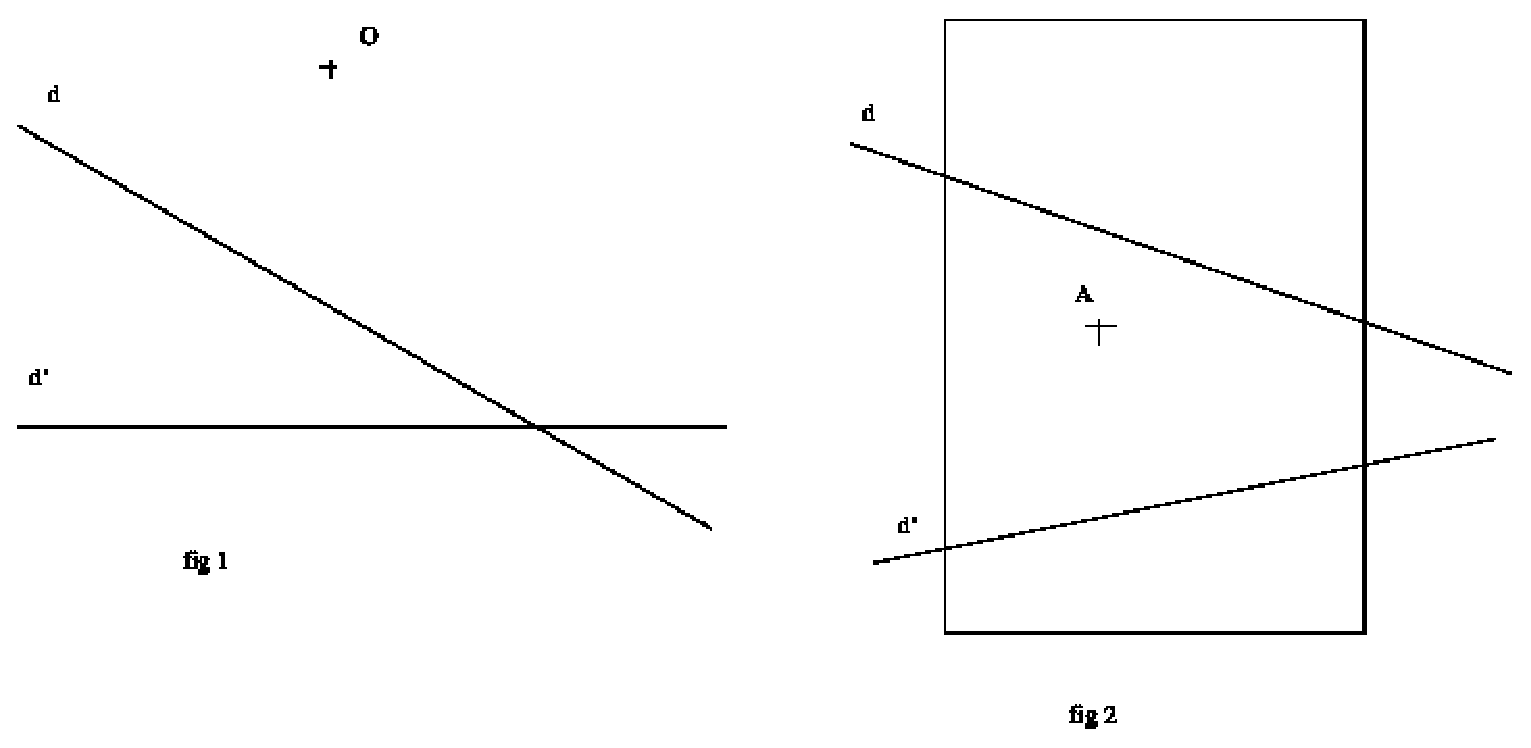
\includegraphics[scale=0.5]{images/img-mour-509}
    %\textit{Justifier votre construction par des arguments de géométrie projective}}
\end{enumerate}
}
